% Created 2021-05-05 Wed 14:54
% Intended LaTeX compiler: pdflatex
\documentclass[11pt]{article}
\usepackage[utf8]{inputenc}
\usepackage{lmodern}
\usepackage[T1]{fontenc}
\usepackage{fixltx2e}
\usepackage{graphicx}
\usepackage{longtable}
\usepackage{float}
\usepackage{wrapfig}
\usepackage{rotating}
\usepackage[normalem]{ulem}
\usepackage{amsmath}
\usepackage{textcomp}
\usepackage{marvosym}
\usepackage{wasysym}
\usepackage{amssymb}
\usepackage{amsmath}
\usepackage[version=3]{mhchem}
\usepackage[numbers,super,sort&compress]{natbib}
\usepackage{natmove}
\usepackage{url}
\usepackage{minted}
\usepackage{underscore}
\usepackage[linktocpage,pdfstartview=FitH,colorlinks,
linkcolor=blue,anchorcolor=blue,
citecolor=blue,filecolor=blue,menucolor=blue,urlcolor=blue]{hyperref}
\usepackage{attachfile}
\usepackage{geometry}
\geometry{margin=1.0in,top=.75in,bottom=.75in}
\usepackage{graphicx}
\usepackage{color}
\usepackage[numbers,super,sort&compress]{natbib}
\usepackage{caption}
\usepackage{subcaption}
\captionsetup{font=footnotesize}
\usepackage[version=3]{mhchem}
\usepackage{siunitx}
\usepackage{fancyhdr}
\usepackage{paralist}
\usepackage{amsmath}
\usepackage{enumitem}
\usepackage{mdwlist}
\usepackage{hyperref}
\pagestyle{fancy}
\usepackage{wrapfig}
\usepackage{nopageno}
\fancyhf{}
\fancyhead[LE,RO]{\scriptsize Jerry Crum}
\fancyhead[RE,LO]{\scriptsize ZSE Outline}
%\fancyfoot[CE,CO]{\leftmark}
\fancyfoot[LE,RO]{\thepage}
%\usepackage{subfig}
\usepackage{comment}
\usepackage{titlesec}
\titlespacing*{\section}
{0pt}{0.6\baselineskip}{0.2\baselineskip}
\titlespacing*{\subsection}
{0pt}{0.6\baselineskip}{0.2\baselineskip}
\titlespacing*{\subsubsection}
{0pt}{0.4\baselineskip}{0.1\baselineskip}
\usepackage{parskip}
\usepackage[section]{placeins}
\usepackage{siunitx}
\DeclareGraphicsExtensions{.pdf,.png,.jpg}
\newcommand{\red}[1]{\textcolor{red}{#1}}
\newcommand{\blue}[1]{\textcolor{blue}{#1}}
\newcommand{\green}[1]{\textcolor{green}{#1}}
\newcommand{\orange}[1]{\textcolor{orange}{#1}}
\usepackage[capitalise]{cleveref}
\author{Jerry T. Crum\(^{\text{a}}\), Justin R. Crum\(^{\text{b}}\), William F. Schneider\(^{\text{a,c}}\)}
\date{}
\title{ZSE Manuscript Outline}
\begin{document}

\begin{OPTIONS}
\def\udesoftecoverride\#1\mainmatter\{\%
  \AfterEndPreamble{#1\mainmatter}
\end{OPTIONS}

\maketitle

\begin{asparaenum}[\expandafter\textsuperscript a ]
\item Department of Chemical and Biolmolecular Engineering, University of Notre Dame, 250 Nieuwland Science Hall, Notre Dame, IN 46556, USA \\
\item Department of Applied Mathematics, University of Arizona, 617 N Santa Rita Ave, Tucson, AZ 85721, USA\\
\item Department of Chemistry and Biochmeistry, University of Notre Dame, 251 Nieuwland Science Hall, Notre Dame, IN 46556, USA
\end{asparaenum}

\newpage
\section*{Introduction}
\label{sec:org8d16b16}
\begin{itemize}
\item Topology of zeolite frameworks and associated tetrahedral sites (T-sites) are commonly characterized by their associated rings
\item Rings are defined as a close cycle traversing the T-site and oxygen atoms of the framework, and cannot be decomposed into smaller cycles by a shortcut \cite{goetzke-properties-1991}.
\item A shortcut is defined as a path connecting two nodes of a cycle that is shorter than both the paths connecting those nodes along the cycle.
\item See \Cref{fig:cha-labeled} for example of rings
\begin{itemize}
\item The pink highlighted cycle (1-2-3-17-20-14-15-16) is a 8-membered ring (8-MR)
\item The green highlighted cycle (14-20-12-13) is a 4-MR
\item The red outlined cycle following 3-4-18-19-20-17 is not an 6-MR because there is a shortcut connecting nodes 17 and 18.
\item Nodes 5-6-7-8-9 outlined in teal represent a path through the framework.
\end{itemize}
\end{itemize}

\begin{center}
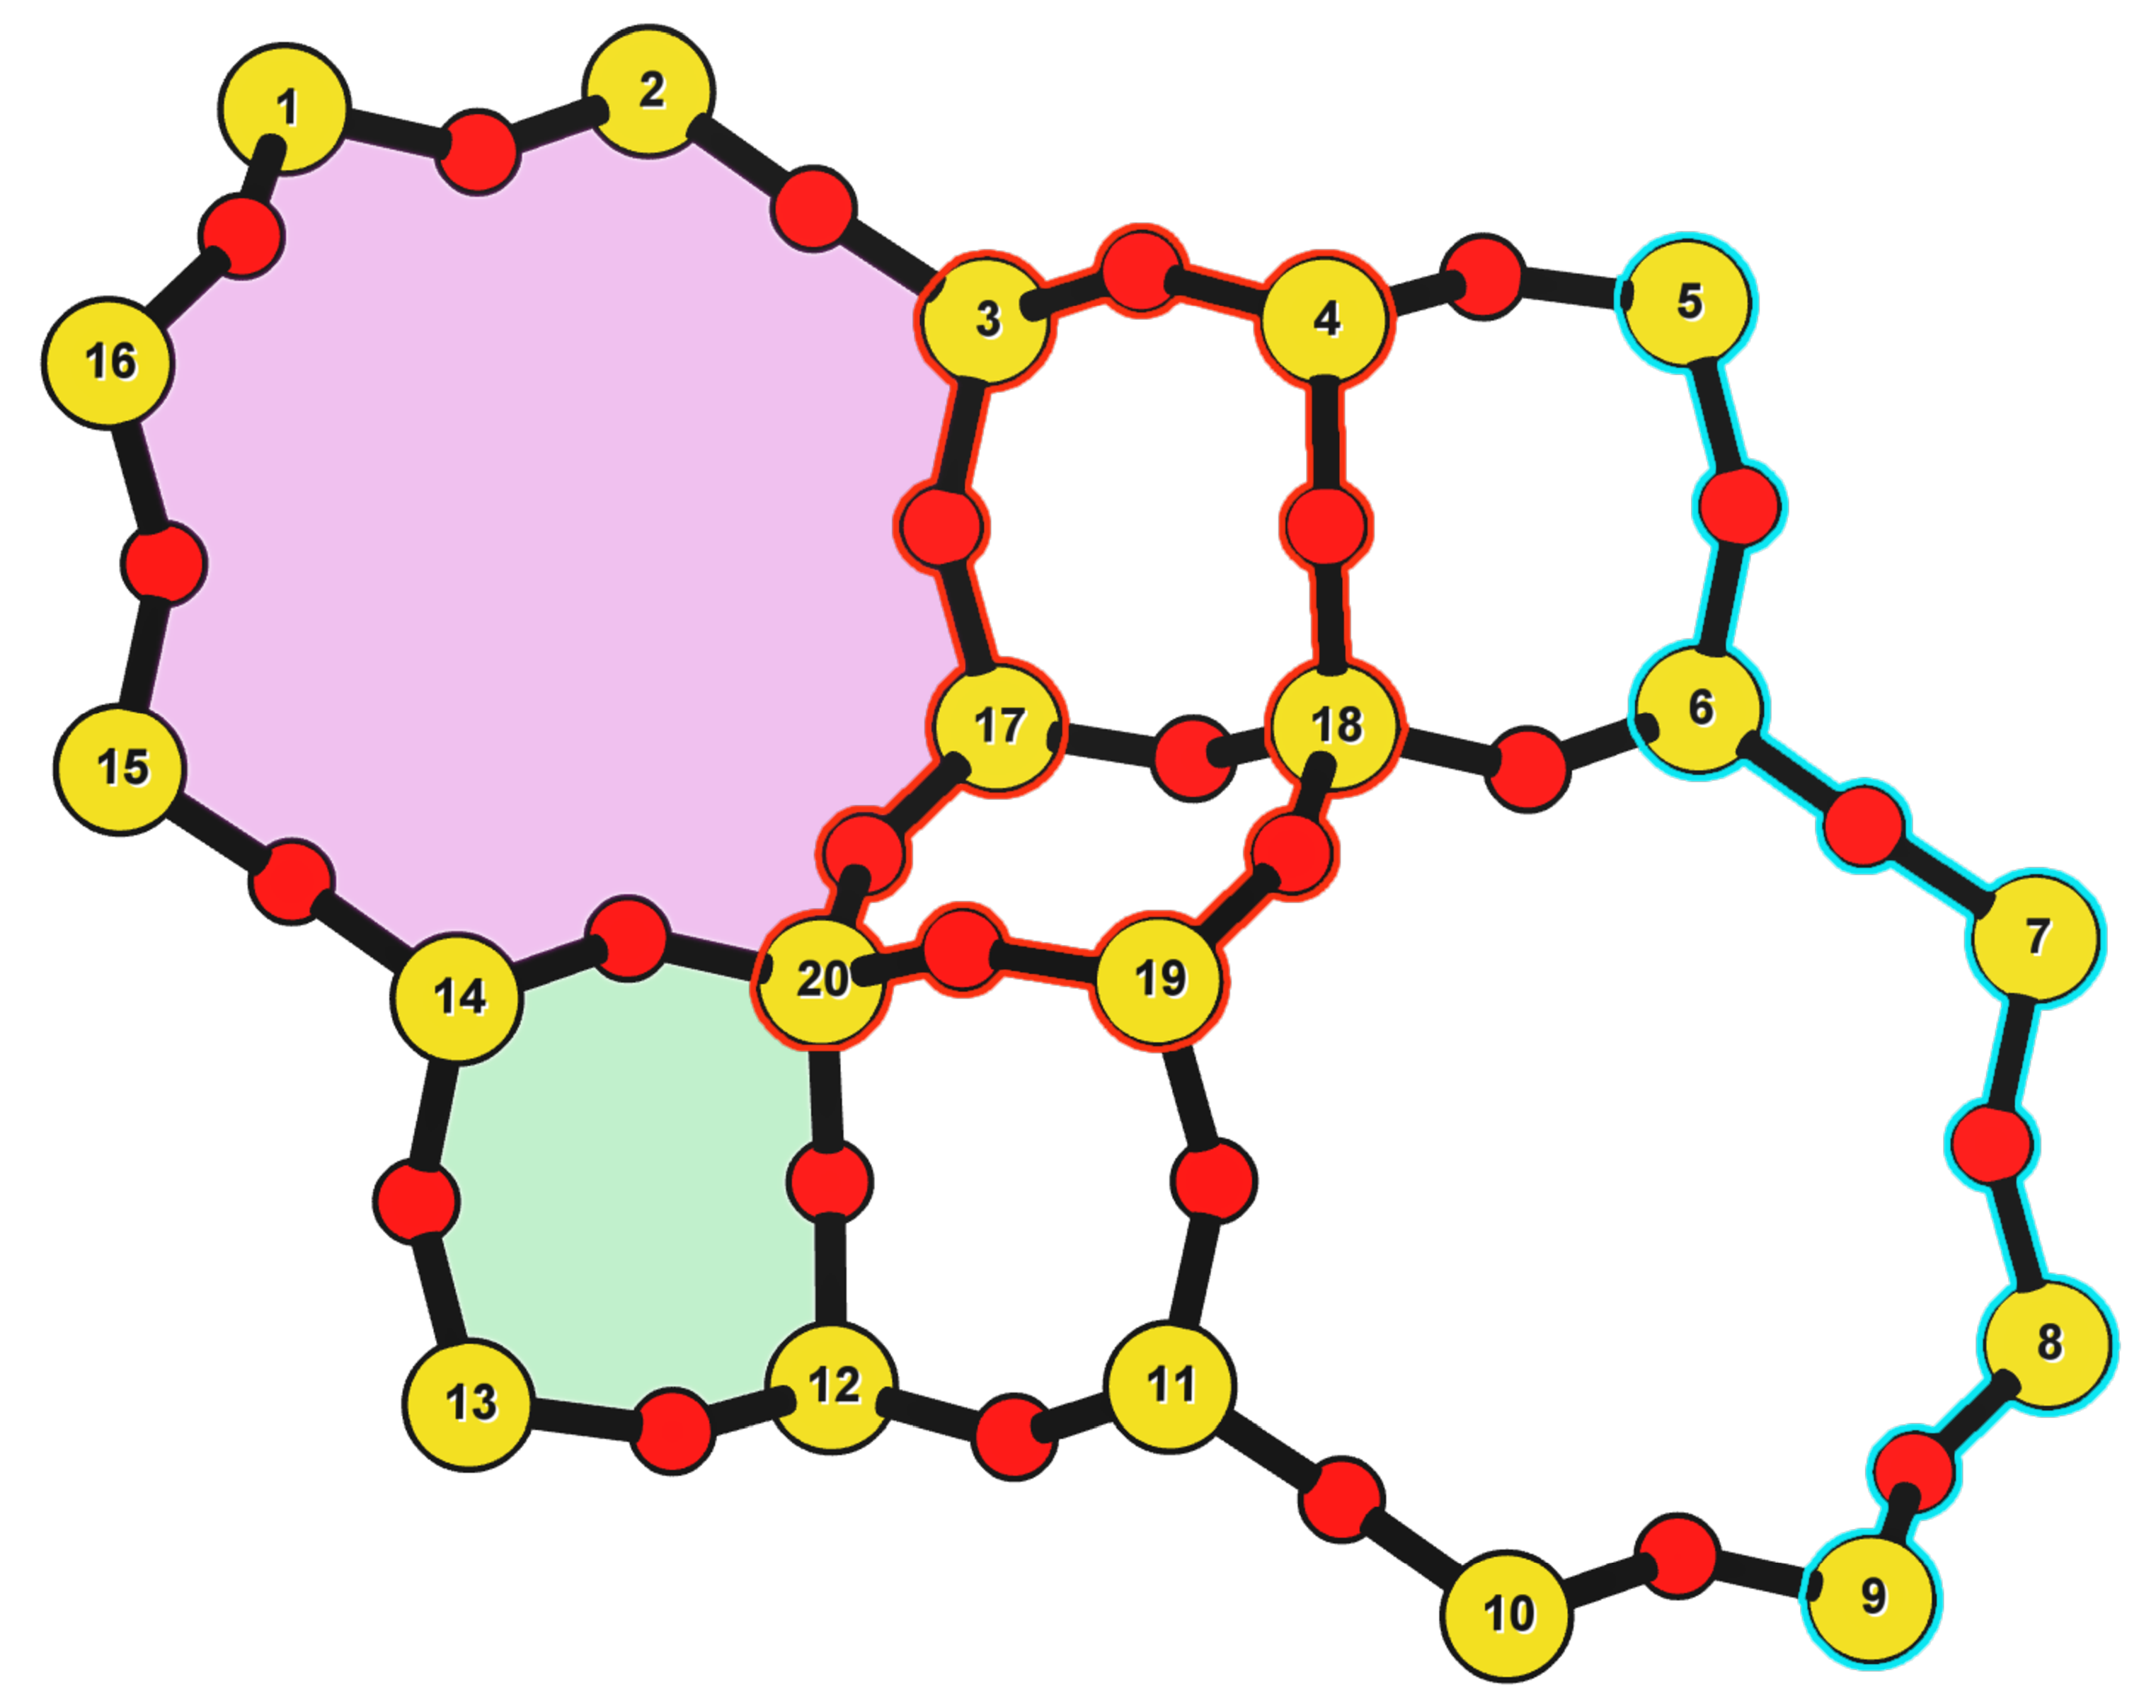
\includegraphics[width=0.60\textwidth]{../figures/completed-figures/ring-examples.pdf}
\captionof{figure}{Cutout of the Chabazite framework showing a path from node 3 to node 9 outlined in teal, a cycle (3-4-18-19-20-17) outlined in red, an 8-MR in pink, and a 4-MR in green. Yellow atoms are Si (T-sites), and red atoms are oxygen. \label{fig:cha-labeled}}
\end{center}
\newpage

\begin{longtable}{l p{2.7cm} p{2.7cm} p{2.7cm} p{2.7cm}}
\caption{Matrix showing relationship between frameoworks, nodes, paths, cycles, and various ring types. \label{tab:ring-def}}
\\
 & Description & Framework & Node (T-Sites) & Node (Oxygen)\\
\hline
\endfirsthead
\multicolumn{5}{l}{Continued from previous page} \\
\hline

 & Description & Framework & Node (T-Sites) & Node (Oxygen) \\

\hline
\endhead
\hline\multicolumn{5}{r}{Continued on next page} \\
\endfoot
\endlastfoot
\hline
Nodes & T-sites and oxygen atoms & Contains some set of symmetry distinct T-sites and oxygen atoms &  & \\
Paths & Collection of connected nodes from source to target & Periodic cell contains an infinite number of paths &  & \\
Cycles & Path that starts and ends at the same node & Periodic cell Contains an infinite number of cycles &  & \\
Rings & Cycle that contains no shortcuts & Contains a finite number of unique rings & All rings that pass through particular T-site & All rings that pass through particular oxygen atom\\
Unstacked Rings & Ring that does not traverse two stacked rings & A subset of the Rings above & All unstacked rings that pass through T-site & All unstacked rings that pass through oxygen atom\\
Shortest Path Rings & Ring that is the shortest ring from at least one set of O-T-O on the cycle & A smaller subset of the rings above & All shortest path rings that pass through T-site & All shortest path rings that pass through oxygen atom\\
Vertex Symbol & Way to classify the rings around a T-site, shortest ring (and its multiplicity) for each O-O pair around a T-site & Collection of vertex symbols for all symmetry distinct T-sites in framework & Vertex symbol for particular T-site & \\
\end{longtable}

\begin{itemize}
\item Rings have been used to identify feasible zeolite topologies \cite{li-why-2014}, to descirbe the similarity and differences between zeolites \cite{curtis-statistical-2003}, to identify sites or voids of catalytic relevance \cite{li-first-principles-2018,kester-effects-2021}, and as machine learning finger prints [will get citations for this]

\item Different methods exist to count rings present in a zeolite
\item These methods return different sets of rings
\item Vertex symbols are the set of shortest paths connecting the 6 oxygen-oxygen pairs around a T-site \cite{okeeffe-vertex-1997}
\item Shortest path rings count all the vertex symbol rings that pass through a T-site or an oxygen atom \cite{sastre-topological-2009}
\item Or we can count all the rings that do not have a short cut \cite{goetzke-properties-1991}
\item Differences in ring counts leads to differences in how we describe the topology of zeolites. Therefore, when discussing the rings in a zeolite it is important to also state which method of ring counting is used.
\item Here we report an analysis of rings and T-sites in a large number of zeolite frameworks using Zeolite Simulation Environment, a Python package that implements an efficient algorithm presented by Goetzke and Klein \cite{goetzke-properties-1991} for finding rings in arbitrary frameworks.
\item We compare the results of a number of common and new ring definitions applied to a large number of common zeolite frameworks.\cite{li-first-principles-2018}
\end{itemize}

\section*{Software Description}
\label{sec:org31f0468}

\begin{itemize}
\item All of the frameworks listed on the IZA Database of zeolite structures \cite{IZA} are included in a database with ZSE
\item These structures are Atomic Simulation Environment Atoms objects \cite{larsen-atomic-2017}, and can be used with any of the functions in ZSE
\item ZSE also includes CIF tools to read structure files for frameworks not listed in the IZA website, such as hypothetical zeolites, and return an Atoms object that can be used with ZSE
\item ZSE has 3 previously published rules for ring finding implemented
\begin{itemize}
\item All cycles with out a shortcut \cite{goetzke-properties-1991}
\item All shortest path cycles \cite{sastre-topological-2009}
\item Cycles that compose the vertex symbol for a T-site \cite{okeeffe-vertex-1997}
\end{itemize}
\item We have also implemented a new rule that finds all rings with out a shortcut, but excludes rings that are made by traversing a stacked set of rings.
\begin{itemize}
\item Figure showing example of 8-MR in the d6r of CHA and 14-MR in AFI
\end{itemize}
\item Each of the rules: shortest path, vertex symbols, and our new rule are a subset of the no shortcuts rule
\end{itemize}
Process to find rings:
\begin{enumerate}
\item To find rings in a zeolite, ZSE makes a custom connectivity matrix for the Si and O atoms in the framework
\item We use NetworkX \cite{SciPyProceedings-11} to build a shortest path matrix for every atom pair in the zeolite framework
\item We then find all the rings up to some cutoff size base on the algorithm presented by Goetzke and Klein \cite{goetzke-properties-1991}
\item Depending on the rule chosen by the user, ZSE then removes rings from this list that don't meet the qualifications of the rule
\item ZSE returns a list of the rings found, a list of the atom indicies that compose each ring, Atoms objects for each ring that can be further analyzed or visualized by the user
\end{enumerate}


\section*{Results}
\label{sec:orgc227a60}
\begin{itemize}
\item Ring counts frequency plots
\begin{itemize}
\item Plot showing how many frameworks on the IZA contain each size ring found using the various ring counting methods
\item This highlights the differences in the ring rules, and shows that results will vary depending on rule.
\end{itemize}
\end{itemize}
\begin{center}
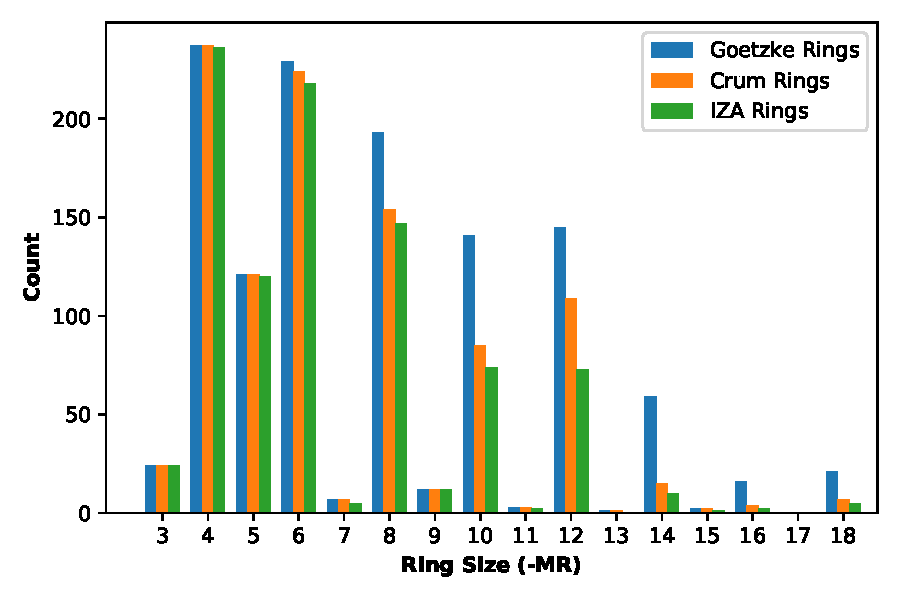
\includegraphics[width=.6\textwidth]{../figures/completed-figures/ring-counts.pdf}
\captionof{figure}{Number of IZA frameworks containing each size ring, using the various ring counting rules. [This will be updated with the Sastre method, vertex method, and the rings listed on  the IZA website. Currently the IZA does not show any ring data for the SVY framework, providing one less framework to count.  \label{fig:ring-counts}}
\end{center}

\begin{itemize}
\item Number of unique T-sites
\begin{itemize}
\item There are 1460 T-sites through all the frameworks listed on the IZA website.
\item We can characterize those T-sites by the rings that pass through them
\item Sastre did this, and called the list of rings, the ring index
\item If we do this using different rules for ring finding how do the results change?
\begin{itemize}
\item See \Cref{fig:unique-ts}
\end{itemize}
\item Most common T-site ring index using Goetzke method is: 5\(_{\text{6}}\)\textbullet{}10\(_{\text{4}}\) showing up 23 times through the IZA frameworks.
\item Most common T-site ring index using Crum method is: 4\(_{\text{3}}\)\textbullet{}8\(_{\text{4}}\) showing up 31 times through the IZA frameworks.
\begin{itemize}
\item Next most common T-site with Crum method is 5\(_{\text{6}}\)\textbullet{}10\(_{\text{4}}\) showing up 25 times
\end{itemize}
\item This raises the question, if you want to use machine learning to correlate T-site rings to chemical properties, which ring method should you use?
\end{itemize}
\end{itemize}
\begin{center}
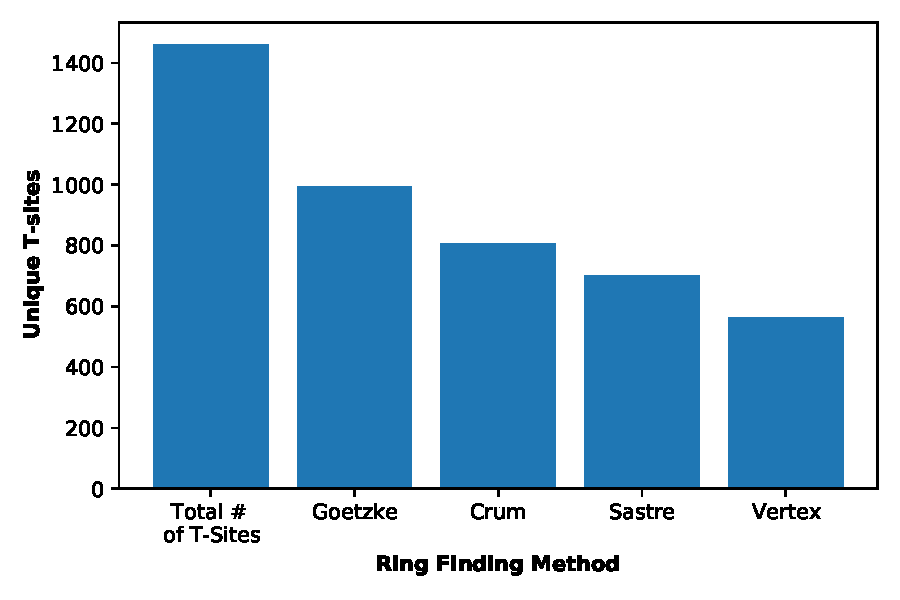
\includegraphics[width=.6\textwidth]{../figures/completed-figures/unique-ts.pdf}
\captionof{figure}{Number of unique T-sites when classified by the rings passing through them using varrious ring finding rules. \label{fig:unique-ts}}
\end{center}

\begin{itemize}
\item Number of unique oxygen sites
\begin{itemize}
\item We can repeat this method for the oxygen atoms in all the frameworks
\item Counting the symmetry distinct oxygen atoms in each framework on the IZA database leads to a total count of 3219
\item We can classify those oxygen atoms based on the rings that pass through them, using the various ring counting rules
\item \Cref{fig:unique-os} shows counts based on ring finding rules
\item The percentage of unique oxygen sites is much lower than the percentage of unique T-sites for every ring finding method
\end{itemize}
\end{itemize}

\begin{center}
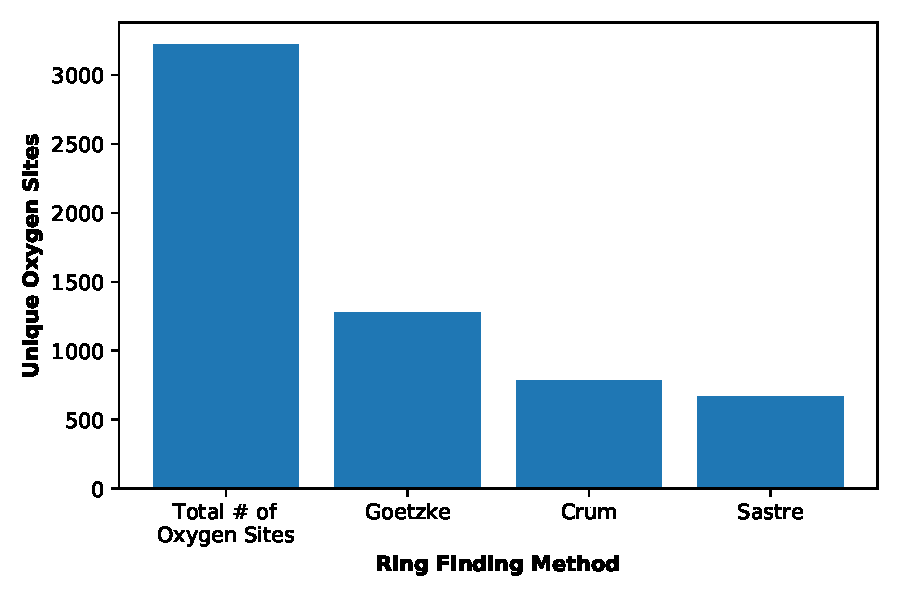
\includegraphics[width=.6\textwidth]{../figures/completed-figures/unique-os.pdf}
\captionof{figure}{Number of unique oxygen sites when classified by the rings passing through them using varrious ring finding rules. Vertex method not included, since that is a way to classify T-sites only. \label{fig:unique-os}}
\end{center}

\begin{itemize}
\item Reproduce the results from Sastre paper, show ring counts with the other rules, \Cref{tab:ring-counts}
\begin{itemize}
\item Results in the Sastre column were found using ZSE but agree directly with the results shown by Sastre and Corma \cite{sastre-topological-2009}
\item This provides an in depth look at some of the frameworks and the differences in rings found by each rule.
\item Leads into the next section discussing the specific rings of CHA and pentasil that do or don't get counted by each rule.
\end{itemize}
\end{itemize}

\begin{table}[htbp]
\caption{Comparison of Ring Indices for the T-sites in Various Uninodal Zeolite Frameworks \label{tab:ring-counts}}
\centering
\begin{tabular}{llll}
Framework & Goetzke & Crum & Sastre \cite{sastre-topological-2009}\\
\hline
ABW & 4\(_{\text{2}}\)\textbullet{}6\(_{\text{3}}\)\textbullet{}8\(_{\text{4}}\) & 4\(_{\text{2}}\)\textbullet{}6\(_{\text{3}}\)\textbullet{}8\(_{\text{4}}\) & 4\(_{\text{2}}\)\textbullet{}6\(_{\text{3}}\)\textbullet{}8\(_{\text{4}}\)\\
ACO & 4\(_{\text{3}}\)\textbullet{}6\(_{\text{3}}\)\textbullet{}8\(_{\text{6}}\)\textbullet{}10\(_{\text{15}}\) & 4\(_{\text{3}}\)\textbullet{}8\(_{\text{6}}\) & 4\(_{\text{3}}\)\textbullet{}8\(_{\text{6}}\)\\
AFI & 4\(_{\text{1}}\)\textbullet{}6\(_{\text{13}}\)\textbullet{}12\(_{\text{1}}\)\textbullet{}14\(_{\text{7}}\) & 4\(_{\text{1}}\)\textbullet{}6\(_{\text{13}}\)\textbullet{}12\(_{\text{1}}\) & 4\(_{\text{1}}\)\textbullet{}6\(_{\text{13}}\)\\
ANA & 4\(_{\text{2}}\)\textbullet{}6\(_{\text{2}}\)\textbullet{}8\(_{\text{16}}\) & 4\(_{\text{2}}\)\textbullet{}6\(_{\text{2}}\)\textbullet{}8\(_{\text{16}}\) & 4\(_{\text{2}}\)\textbullet{}6\(_{\text{2}}\)\textbullet{}8\(_{\text{16}}\)\\
ATO & 4\(_{\text{1}}\)\textbullet{}6\(_{\text{9}}\)\textbullet{}8\(_{\text{8}}\)\textbullet{}12\(_{\text{20}}\) & 4\(_{\text{1}}\)\textbullet{}6\(_{\text{9}}\)\textbullet{}12\(_{\text{20}}\) & 4\(_{\text{1}}\)\textbullet{}6\(_{\text{9}}\)\\
BCT & 4\(_{\text{1}}\)\textbullet{}6\(_{\text{6}}\)\textbullet{}8\(_{\text{20}}\) & 4\(_{\text{1}}\)\textbullet{}6\(_{\text{6}}\)\textbullet{}8\(_{\text{12}}\) & 4\(_{\text{1}}\)\textbullet{}6\(_{\text{6}}\)\\
CHA & 4\(_{\text{3}}\)\textbullet{}6\(_{\text{1}}\)\textbullet{}8\(_{\text{6}}\)\textbullet{}12\(_{\text{1}}\) & 4\(_{\text{3}}\)\textbullet{}6\(_{\text{1}}\)\textbullet{}8\(_{\text{2}}\)\textbullet{}12\(_{\text{1}}\) & 4\(_{\text{3}}\)\textbullet{}6\(_{\text{1}}\)\textbullet{}8\(_{\text{2}}\)\\
DFT & 4\(_{\text{2}}\)\textbullet{}6\(_{\text{6}}\)\textbullet{}8\(_{\text{10}}\)\textbullet{}10\(_{\text{10}}\) & 4\(_{\text{2}}\)\textbullet{}6\(_{\text{6}}\)\textbullet{}8\(_{\text{10}}\) & 4\(_{\text{2}}\)\textbullet{}6\(_{\text{6}}\)\textbullet{}8\(_{\text{10}}\)\\
GIS & 4\(_{\text{3}}\)\textbullet{}8\(_{\text{4}}\) & 4\(_{\text{3}}\)\textbullet{}8\(_{\text{4}}\) & 4\(_{\text{3}}\)\textbullet{}8\(_{\text{4}}\)\\
GME & 4\(_{\text{3}}\)\textbullet{}6\(_{\text{1}}\)\textbullet{}8\(_{\text{6}}\)\textbullet{}12\(_{\text{7}}\) & 4\(_{\text{3}}\)\textbullet{}6\(_{\text{1}}\)\textbullet{}8\(_{\text{2}}\)\textbullet{}12\(_{\text{1}}\) & 4\(_{\text{3}}\)\textbullet{}6\(_{\text{1}}\)\textbullet{}8\(_{\text{2}}\)\\
MER & 4\(_{\text{3}}\)\textbullet{}8\(_{\text{4}}\)\textbullet{}10\(_{\text{10}}\)\textbullet{}14\(_{\text{14}}\) & 4\(_{\text{3}}\)\textbullet{}8\(_{\text{4}}\) & 4\(_{\text{3}}\)\textbullet{}8\(_{\text{4}}\)\\
MON & 4\(_{\text{1}}\)\textbullet{}5\(_{\text{5}}\)\textbullet{}8\(_{\text{6}}\) & 4\(_{\text{1}}\)\textbullet{}5\(_{\text{5}}\)\textbullet{}8\(_{\text{6}}\) & 4\(_{\text{1}}\)\textbullet{}5\(_{\text{5}}\)\textbullet{}8\(_{\text{6}}\)\\
NPO & 3\(_{\text{1}}\)\textbullet{}6\(_{\text{6}}\)\textbullet{}12\(_{\text{40}}\) & 3\(_{\text{1}}\)\textbullet{}6\(_{\text{6}}\)\textbullet{}12\(_{\text{40}}\) & 3\(_{\text{1}}\)\textbullet{}6\(_{\text{6}}\)\\
\end{tabular}
\end{table}

\begin{itemize}
\item Show the cage belts results for CHA, AFT, etc\ldots{} and discuss how those rings don't show up in previous literature, \Cref{fig:cha-rings}
\begin{itemize}
\item Looking at results from CHA we see the Goetzke method finds 4\(_{\text{3}}\)\textbullet{}6\(_{\text{1}}\)\textbullet{}8\(_{\text{6}}\)\textbullet{}12\(_{\text{1}}\)
\item This is different from the results in the Sastre paper \cite{sastre-topological-2009}, in that they only show 2 8-MRs and no 12-MRs
\item The extra 8-MRs result from cycles traversing nodes in both 6-MRs of the d6r
\item The 12-MR is a cycle that circumferences the CHA cage
\end{itemize}
\end{itemize}
\begin{center}
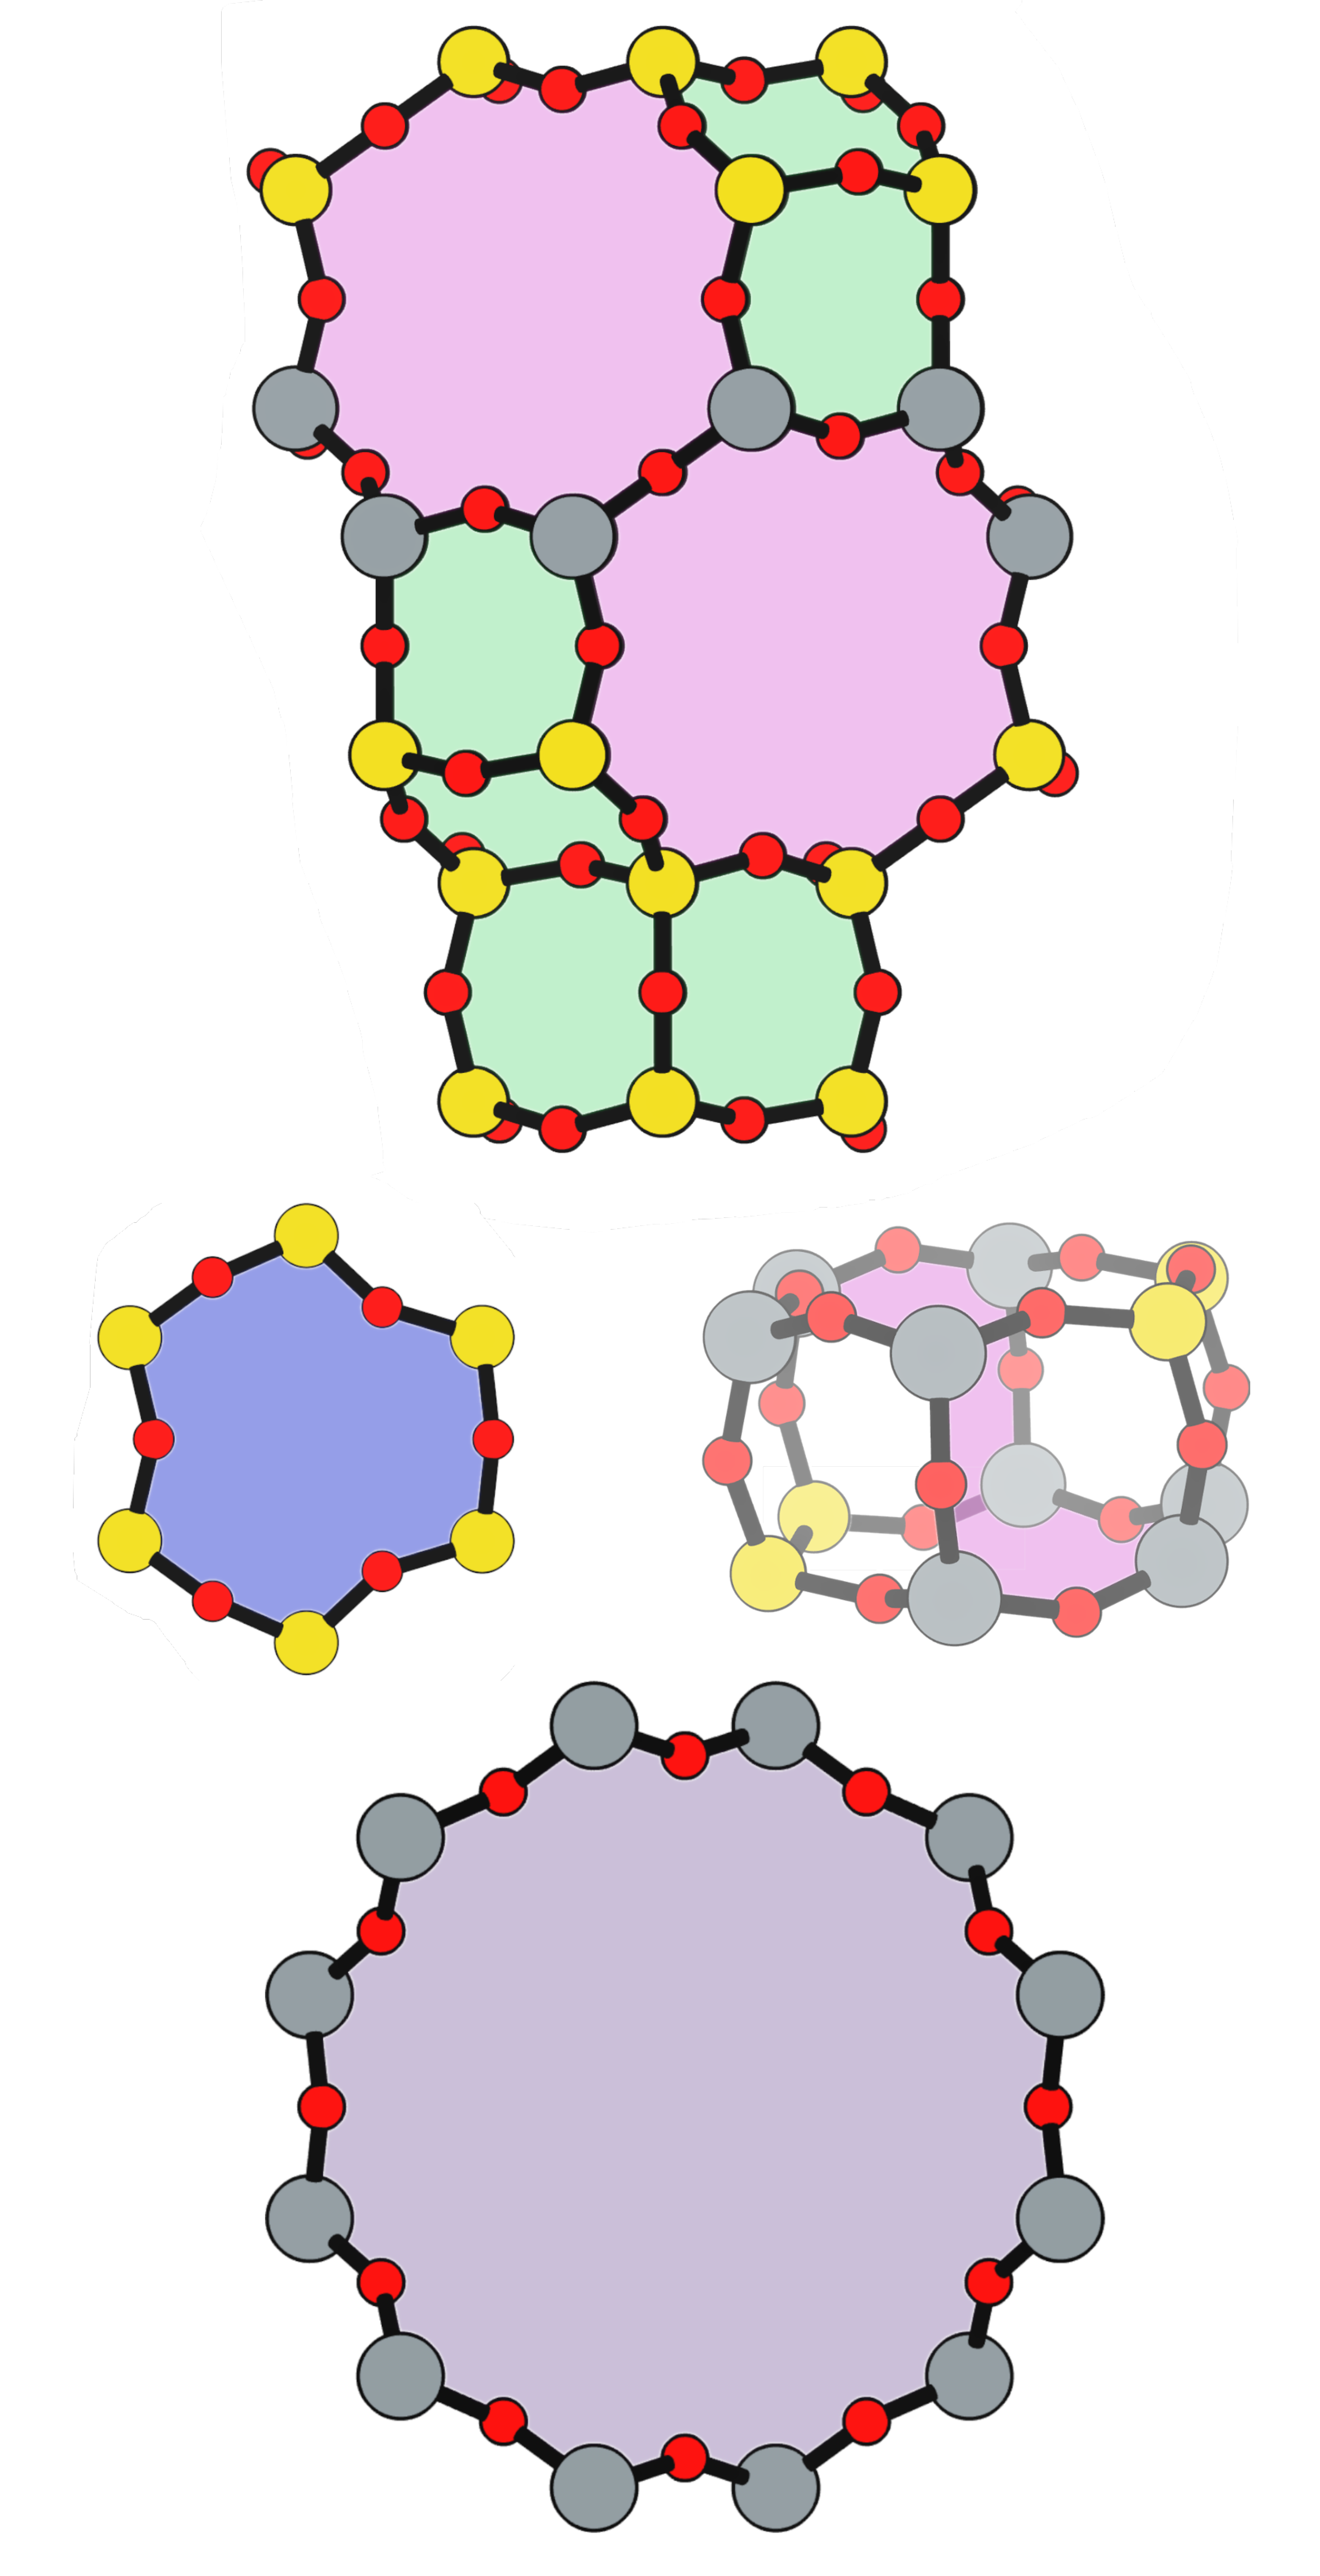
\includegraphics[width=0.45\textwidth]{../figures/completed-figures/cha-all-rings.pdf}
\captionof{figure}{Chabazite framework with highlighted rings: 4-MR in green, 6-MR in blue, 8-MR in pink, 12-MR in purple. The 8-MR in the d6r and the 12-MR are rings not typically discussed in literature. This is a placeholder figure, I want to show the rings in CHA for discussion. Hoping to get your input on how best to do that. \label{fig:cha-rings}}
\end{center}

\begin{itemize}
\item Show the pentasil 6-membered cycle (MFI) and discuss how that is often considered a ring by catalysis researchers, but not a ring by the Goetzke definition
\end{itemize}

\section*{Conclusions}
\label{sec:org6e9315d}

\begin{itemize}
\item The method used to find rings in a zeolite will provide different ring counts
\item When discussing rings in a zeolite it is import to disclose by which method those rings were found
\item Using ZSE we can find rings based on various methods
\item This provides a foundation for using ring fingerprints in machine learning models to correlate chemical properties and topology
\end{itemize}


\bibliographystyle{unsrtnat}
\bibliography{ref}
\end{document}